\documentclass[a4paper, 12pt]{article}

%Русский язык
\renewcommand{\familydefault}{\sfdefault}%шрифт
\usepackage[T2A]{fontenc} %кодировка
\usepackage[utf8]{inputenc} %кодировка исходного кода
\usepackage[english,russian]{babel} %локализация и переносы
%отступы 
\usepackage[left=2cm,right=2cm,top=2cm,bottom=3cm,bindingoffset=0cm]{geometry}
\usepackage{indentfirst}
%Вставка картинок
\usepackage{graphicx}
\graphicspath{}
\DeclareGraphicsExtensions{.pdf,.png,.jpg, .jpeg}

%Таблицы
\usepackage[table,xcdraw]{xcolor}
\usepackage{booktabs}

% Cсылки
\usepackage{hyperref}
\bibliographystyle{unsrt}
%Математика
\usepackage{physics}
\usepackage{amssymb}
% \DeclareMathOperator*{\Res}{Res}
\DeclareMathOperator*{\sign}{sign}
\DeclareMathOperator*{\Real}{Re}
\DeclareMathOperator*{\Imag}{Im}

%%Окружение для многострочных уравнений
\newenvironment{eqw}{\begin{equation} \begin{aligned}}   
    {\end{aligned}    \end{equation}}
\newenvironment{eqw*}{\begin{equation*} \begin{aligned}}   
    {\end{aligned}    \end{equation*}}
%Заголовок
\author{Нугманов Булат}
\title{Математическое приложение}
\begin{document}
\maketitle
Данный документ является наброском математического приложения, результаты которого точно выполняются численно. А ещё надо будет это перевести.

\begin{enumerate}
    \item Переписывание ряда через интеграл
    \item Нахождение перевальных точек
    \item Асимптотика кривых постоянной фазы через перевальные точки --- \textcolor{red}{не знаю, надо ли об этом писать?}
    \item Деформация контура в зависимости от знака $\Gamma$ --- \textcolor{red}{пока нет}
    \item Подсчёт вкладов по методу перевала
    \item Вставка с полиномами Белла и числами Стирлинга для явного подсчёта коэффициентов в методе перевала
    \item Слова о том, что при $|\Gamma| \ll 1$ достаточно учитывать лишь одно слагаемое
    \item Точное значение в максимуме
    \item Выбор $\overline{k}$
    \item Граница выбора $\overline{k}$
    \item Итог: асимптотика ряда
\end{enumerate}
\section*{Вступление}
In this section we will find the asymptotics of the series of the following form:
\begin{eqw}\label{F def}
    F(A, e^{i\Gamma}) = \sum\limits_{n=0}^{\infty} \frac{A^n e^{i\Gamma n^2}}{n!},
\end{eqw}
when $\Gamma\in \mathbb{R}$, $A\in \mathbb{C}$ and $|\Gamma| \ll 1$. 

Наметим примерный план дальнейшего рассказа. Первым делом мы перейдём от суммы к расчёту интеграла по действительной оси. Далее мы воспользуемся отсутствием полюсов подынтегральной функции и деформируем контур так, чтоб он проходил через перевальные точки по кривым постоянной фазы. 
После этого математическая мысль может двигаться в двух направлениях. С одной стороны мы можем строго вывести все остаточные члены, используя формулу CFWW и ассоциированные числа Стирлинга. С другой стороны мы можем использовать то, что при $|\Gamma| \ll 1$ основной вклад в получившуюся сумму вносит лишь одно слагаемое с номером $\bar k$. Можно воспользоваться приближёнными вычислениями для определения $\bar k$, а далее можно найти простую асимптотику при $|A\Gamma|\gg1$. Эти направления мысли почти не связаны. И если первая служит больше для теоретической полноты описания, то вторая больше служит для численных расчётов. 

\section*{Переход от суммы к интегралу}
Вычисление суммы "табличными" методами существенно осложняется множителем $\exp\left(i\Gamma n^2\right)$. Воспользуемся следующей формулой (здесь и далее мы будем подразумевать все интегралы в смысле главного значения):
\begin{eqw}
    \exp\left(i\Gamma n^2\right) = \frac{e^{i\frac{\pi}{4}\sign \Gamma}}{2\sqrt{\pi|\Gamma|}}
    \int\limits_{-\infty}^{\infty} \exp\left(-\frac{i z^2}{4\Gamma} + i n z\right) dz
\end{eqw}
Применим данную формулу для ряда \eqref{F def}:
\begin{eqw}
    \sum\limits_{n=0}^{\infty} \frac{A^n e^{i\Gamma n^2}}{n!} = \frac{e^{i\frac{\pi}{4}\sign \Gamma}}{2\sqrt{\pi|\Gamma|}}
    \int\limits_{-\infty}^{\infty} \exp\left(-\frac{i z^2}{4\Gamma} +  A e^{iz}\right) dz
\end{eqw}
Приведём данную формулу к более удобному для применения метода перевала виду. Для этого введём обозначения
\begin{eqw}
    f(z) =  \frac{z^2}{2i} + i Z e^{iz}\\
    Z = -2i A \Gamma = R e^{i\Phi},
\end{eqw}
где $\Phi\in\left(-\pi, \pi\right]$ и $R\in\mathbb{R}$. И наконец, 
\begin{eqw}\label{row to integral}
    \sum\limits_{n=0}^{\infty} \frac{A^n e^{i\Gamma n^2}}{n!} = \frac{e^{i\frac{\pi}{4}\sign \Gamma}}{2\sqrt{\pi|\Gamma|}}
    \int\limits_{-\infty}^{\infty}\exp\left(\frac{f(z)}{2\Gamma}\right)dz 
\end{eqw}

\section*{Применение метода перевала}
\subsection*{Перевальные точки}
Начнём с поиска перевальных точек, которые являются решением $f'(z)=0$. Бесконечное множество таких решений можно занумеровать номером $k$:
\begin{eqw}
    e^{i z_k} = \frac{z_k}{iZ} \Rightarrow   z_k = i W_k(Z),
\end{eqw}
где $W_k$ --- $k$-ая ветвь $W$-функции Ламберта. 
\subsection*{Деформация контура через кривые постоянной фазы}
\begin{figure}
    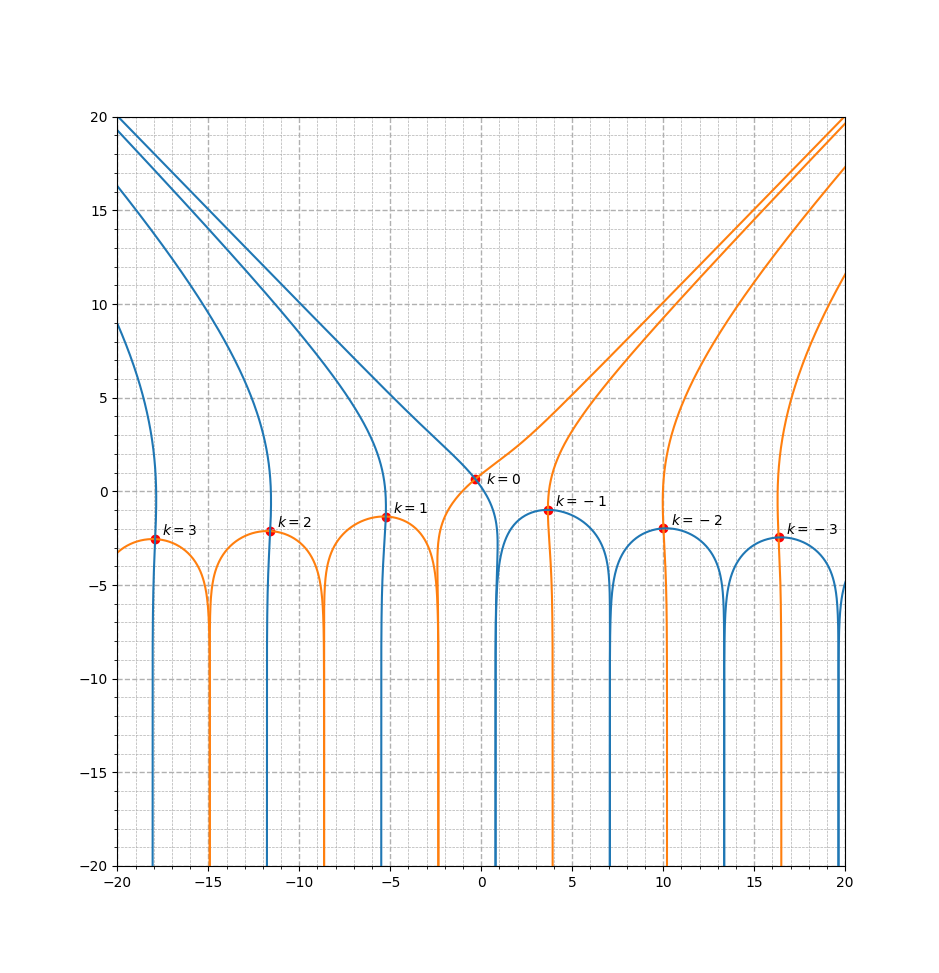
\includegraphics[width=\textwidth]{constant_phase_curve.png}
    \caption{Кривые постоянной фазы для интеграла \ref{row to integral} при $Z=1+i$. Синим указаны кривые наискорейшего спуска $\gamma_k$ при $\Gamma < 0$, оранжевым --- при $\Gamma > 0$. Красные точки пересечения кривых --- точки перевала $f'(z_k)=0$.}
\end{figure}
\textcolor{red}{Здесь должно быть объяснение того, почему мы выбриаем только некоторые из всего множества точек. График с положением перевальных точек, кривыми постоянных фаз через каждую из точек, доказательство того, что номера выбора перевальных точек должны быть инвариантны относительно $Z$ и пара слов про расходимость теории при особом случае $Z=-e^{-1}$. А ещё пара слов о том, почему контур действительно деформируется и удалённых областях интеграл по дополнительным (непервальным) контурам стремится к нулю.}

Правильно выбрав контура интегрирования $\gamma_k$, мы можем сформулировать следующее:
\begin{eqw}\label{contour deformation}
    \int\limits_{-\infty}^{\infty}\exp\left(\frac{f(z)}{2\Gamma}\right) dz = \sum\limits_{k=0}^{-\sign\Gamma \cdot \infty}
    \int\limits_{\gamma_k} \exp\left(\frac{f(z)}{2\Gamma}\right) dz
\end{eqw}
\section*{Интеграл по $\gamma_k$}
Для расчёта интеграла вдоль некоторой $\gamma_k$, мы воспользуемся формулой CFWW \cite{bleistein1975asymptotic}. Для её применения нам необходимо разложение в ряд Тейлора функции $f$ в окрестности перевальной точки:
\begin{eqw}\label{f taylor}
    f(z) = \underbrace{\frac{z_k^2}{2i} + z_k}_{f(z_k)} + \underbrace{\frac{-i-z_k}{2}}_{a_0} (z-z_k)^2 + 
    \sum_{n=1}^{\infty} \underbrace{\frac{-i^n z_k}{(n+2)!}}_{a_1, \: a_2, \dots} (z-z_k)^{n+2}
\end{eqw}
Для использовании CFWW мысленно разделим контур интегрирования на две части, начинающиеся в $z_k$ уходящие на бесконечность. Учитывая, что перевальная точка имеет второй порядок\footnote{Особый случай $z_k = -i$ или, что то же самое $W_k(Z) = -1$ соответствует точке ветвления $W$-функции Ламберта. При этом $Z=-e^{-1}$, а перевальные точки соответствующие $k=-1, 0, 1$ схлопываются в одну. Мы не будем рассматривать этот крайне редкий случай.}, запишем итоговый результат:
\begin{eqw}\label{asymptotic gamma_k int raw}
    \int\limits_{\gamma_k} \exp\left(\frac{f(z)}{2\Gamma}\right) dz 
    &= \exp\left(\frac{ f(z_k)}{2\Gamma} \right)\sqrt{\frac{2\Gamma}{a_0}}\sum\limits_{n=0}^{\infty} 
    \Gamma\left(n+\frac{1}{2}\right)\left(2\Gamma\right)^n c_{2n}\\
    c_{2n} &= \sum\limits_{j=0}^{2n} \frac{C_{-n-\frac{1}{2}}^j}{a_0^{n+j}}\hat{B}_{2n, j}\left(a_1, a_2, \dots, a_{2n-j+1}\right),
\end{eqw}
где $\hat{B}_{2n, j}\left(a_1, a_2, \dots, a_{2n-j+1}\right)$ --- экспоненциальные полиномы Белла от коэффициентов в разложении  $f$ по ряду Тейлора \eqref{f taylor}. 

\subsection*{Полиномы Белла}
Полиномы Белла задаются имеют производящую функцию:
\begin{eqw}\label{Bell generating func}
    \exp\left(u \sum\limits_{j=1}^{\infty}x_j t^j\right) = \sum\limits_{n\geq k\geq 0} 
    \hat{B}_{n,k}\left(x_1, x_2, \dots, x_{n-k+1}\right) t^n \frac{u^k}{k!}
\end{eqw}
Из этого определения легко можно вывести:
\begin{eqw}
    \hat{B}_{2n, j}(\zeta x_1, \zeta x_2, \dots, \zeta x_{2n-j+1}) &= \zeta^j \hat{B}_{2n, j}( x_1,  x_2, \dots,  x_{2n-j+1})\\
    \hat{B}_{2n, j}(\zeta x_1, \zeta^2 x_2, \dots, \zeta^{2n-j+1} x_{2n-j+1}) &= \zeta^{2n} \hat{B}_{2n, j}( x_1,  x_2, \dots,  x_{2n-j+1})
\end{eqw}
Применим эти формулы для полиномов Белла, встречающихся в \eqref{asymptotic gamma_k int raw}:
\begin{eqw}\label{Bell simplification}
    \hat{B}_{2n, j}\left(a_1, a_2, \dots, a_{2n-j+1}\right) &= 
    \hat{B}_{2n, j}\left(\frac{-i z_k}{3!}, \frac{-i^2 z_k}{4!}, \dots, \frac{-i^{2n-j+1} z_k}{(2n-j+3)!}\right) \\
    &= (-1)^n(-z_k)^{j}\hat{B}_{2n, j}\left(\frac{1}{3!}, \frac{1}{4!}, \dots, \frac{1}{(2n-j+3)!}\right)
\end{eqw}

\section*{Связь полиномов Белла и чисел Стирлинга}
В данном разделе мы докажем следующую формулу:
\begin{eqw}\label{Bell and Stirling connection}
    \hat{B}_{n, k}\left(\frac{1}{r!}, \frac{1}{(r+1)!}, \dots, \frac{1}{(n-k+r)!}\right) = 
    \frac{k!}{(n+(r-1)k)!}S_{r}(n+(r-1)k, k)
\end{eqw}
где далее можно использовать рекуррентную формулу \cite[~p. 222]{comtet2012advanced}
\begin{eqw}
    S_r(n+1, k) = k S_r(n, k) + C_n^{r} S_r(n-r+1, k-1)
\end{eqw}

\subsection*{Доказательство}
Ассоциированные числа Стирлинга имеют следующее определение \cite[~p. 222]{comtet2012advanced}
\begin{eqw}\label{Stirling generating func}
    \exp\left(u\left(\frac{t^r}{r!}+\frac{t^{r+1}}{\left(r+1\right)!}+\dots\right)\right) = \sum\limits_{n=(r+1)k, k = 0}^{\infty} S_{r}(n, k) u^k \frac{t^n}{n!}
\end{eqw}

Сравнивая производящую функцию чисел Стирлинга \eqref{Stirling generating func} и полиномов Бернулли \eqref{Bell generating func}, можно заметить некоторое сходство:
\begin{eqw}
    \sum\limits_{n\geq k\geq 0} 
    \hat{B}_{n, k}&\left(\frac{1}{r!}, \frac{1}{(r+1)!}, \dots, \frac{1}{(n-k+r)!}\right) t^n \frac{u^k}{k!} = 
    \exp\left(\frac{u}{t^{r-1}} \left(\frac{t^r}{r!} + \frac{t^{r+1}}{(r+1)!}+\dots \right)\right) \\ 
    &= \sum\limits_{n, k}^{\infty} S_{r}(n, k) \frac{u^k}{t^{(r-1)k}}\frac{t^n}{n!} \\
    &= \sum\limits_{n, k}^{\infty} S_{r}(n+(r-1)k, k) u^k\frac{t^n}{(n+(r-1)k)!}
\end{eqw}
Сравнивая первую и последнюю строчку полученного выражения получаем требуемое \eqref{Bell and Stirling connection}.
\section*{Точная формула}
Собирая воедино формулы \eqref{asymptotic gamma_k int raw}, \eqref{Bell simplification}, \eqref{Bell and Stirling connection} приходим к следующему:
\begin{eqw}
    &\Gamma\left(n+\frac{1}{2}\right) c_{2n} =
    \Gamma\left(n+\frac{1}{2}\right) \sum\limits_{j=0}^{2n} C_{-n-\frac{1}{2}}^j\frac{1}{a_0^{n+j}}
    \hat{B}_{2n, j}\left(a_1, a_2, \dots, a_{2n-j+1}\right) \\
    &\;\;\;\;\; = 
    \sum\limits_{j=0}^{2n} \frac{\Gamma\left(n+\frac{1}{2}\right)\Gamma\left(-n+\frac{1}{2}\right)}{j!\Gamma\left(-n-j+\frac{1}{2}\right)}
    \frac{1}{\left(\frac{-i-z_k}{2}\right)^{n+j}}
    (-1)^n (-z_k)^j\hat B_{2n, j}\left(\frac{1}{3!}, \frac{1}{4!}, \dots, \frac{1}{(2n-j+3)!}\right)\\
    &\;\;\;\;\; = 
    \sum\limits_{j=0}^{2n} \frac{\frac{\pi}{\sin\left(\pi n + \frac{\pi}{2}\right)}}{j!\frac{(-4)^{n+j}(n+j)!}{(2n+2j)!}\sqrt{\pi}}
    \frac{(-1)^n (-z_k)^j}{\left(\frac{-i-z_k}{2}\right)^{n+j}} \frac{j!}{(2n+2j)!}S_3(2n+2j, j)\\
    &\;\;\;\;\; = 
    \sum\limits_{j=0}^{2n} \frac{\sqrt{\pi}}{(-4)^{n+j}(n+j)!}
    \frac{(-z_k)^j}{\left(\frac{-i-z_k}{2}\right)^{n+j}} S_3(2n+2j, j) = 
    \frac{\sqrt{\pi}}{2^n(i+z_k)^n}
    \sum\limits_{j=0}^{2n} \left(-\frac{1}{2}\frac{z_k}{i+z_k}\right)^{j}\frac{S_3(2n+2j, j)}{(n+j)!}
\end{eqw}

Подставляя этот результат в \eqref{row to integral}, \eqref{contour deformation}, находим:
\begin{eqw}
    \sum\limits_{n=0}^{\infty}\left(\frac{iZ}{2\Gamma}\right)^n  \frac{e^{i\Gamma n^2}}{n!} &= e^{\frac{i\pi}{4}\sign\Gamma}
    \sum\limits_{k=0}^{-\sign\Gamma\cdot\infty} \frac{\exp\left(\frac{-i-i(z_k+i)^2}{4\Gamma}\right)}{\sqrt{-\sign \Gamma\left(i+z_k\right)}}
    \times\dots\\
    &\dots\times
    \sum\limits_{n=0}^{\infty}\left(\frac{\Gamma}{i+z_k}\right)^n
    \sum\limits_{j=0}^{2n}\left(-\frac{1}{2}\frac{z_k}{i+z_k}\right)^{j}\frac{S_3(2n+2j, j)}{(n+j)!},
\end{eqw}
где выбор ветви корня определяется из условия:
\begin{eqw}
    \arg\sqrt{-\sign \Gamma\left(i+z_k\right)} \in \left(-\frac{\pi}{2}, \frac{\pi}{2}\right)
\end{eqw}
Такое условие обусловлено направлением $\gamma_k$ в точке перевала. И так как изначальный интеграл \eqref{row to integral} брался в пределах $(-\infty, \infty)$, то $\gamma_k$ так же имеет направление слева направо. 

\textcolor{red}{Если сделать нормальное пояснение картинок $\gamma_k$ в разделе про деформацию контура, то здесь всё станет понятно и очевидно...}


\section*{Наилучшее $\bar k$}
Далее мы переходим к менее точным оценкам.
\begin{eqw}\label{approx_exact_row}
    \left|\sum\limits_{n=0}^{\infty}\left(\frac{iZ}{2\Gamma}\right)^n  \frac{e^{i\Gamma n^2}}{n!} \right|\approx 
    \frac{\exp\left(\frac{-i-i(z_{\bar k}+i)^2}{4\Gamma}\right)}{\left|i+z_{\bar k}\right|^{\frac{1}{2}}}
\end{eqw}
Выпишем действительную часть показателя экспоненты:
\begin{eqw}\label{real f z k through W}
    \Real\left(f(z_k)\right) = \frac{1}{2}\Real\left(-i(z_k+i)^2\right) = -\Imag(W_k(Z))\left(1+\Real(W_k(Z))\right)
\end{eqw}
\subsection*{Точное поведение $\Real f(z_k)$}
Рассмотрим функцию $\Real f(iW(R e^{i\Phi}))$ как функцию от $\Phi\in(-\infty, \infty)$, учитывая, что при изменении $\Phi$ на $2\pi$ меняется ветвь $W$-функции Ламберта. (Для сокращения дальнейших формул используем в данном параграфе сокращение $W = W(Z=R e^{i\Phi})$). Найдём максимум функции $\Real f(iW(R e^{i\Phi}))$ от $\Phi$.  Для этого нам понадобиться формула для производной \cite[formula 3.2]{corless1996lambertw}:

\begin{eqw}
    \frac{\partial W}{\partial \Phi} = \frac{iW}{1+W}
\end{eqw}
Подставляя это выражение в \eqref{real f z k through W}:
\begin{eqw}
    \frac{\partial}{\partial\Phi}\Real\left(f(z_k)\right) = -\Real(W)
\end{eqw}

В точке максимума $\frac{\partial}{\partial\Phi}\Real\left(f(z_k)\right) = 0$. Отсюда из определения $W$-функции Ламберта
\begin{eqw}
    i\Imag W e^{i\Imag W} = R e^{i\Phi_{\max}} \Rightarrow \left|\Imag W\right| = R
\end{eqw}
Неопределённость знака $\Imag W$ можно снять, если учесть, что мы ищем именно максимум, а не произвольный экстремум:
\begin{eqw}
    \sign\left(\frac{f(z_k)}{2\Gamma}\right)_{\Phi = \Phi_{max}} = 1 \Rightarrow \Imag W = - R\sign \Gamma 
    &\Rightarrow \left(\frac{f(z_k)}{2\Gamma}\right)_{\Phi = \Phi_{max}} = \frac{R}{2|\Gamma|}
\end{eqw}
Используя определение $W$-функции Ламберта, находим $\Phi_{\max}$:
\begin{eqw}
    - i R \sign \Gamma  e^{- i R \sign \Gamma } = R e^{i\Phi_{\max}} &\Rightarrow \Phi_{\max} = -\left(R+\frac{\pi}{2}\right)\sign \Gamma \;\;\; \mod 2\pi
\end{eqw}
Взятием производных более высоких порядков \cite[formula 3.5]{corless1996lambertw} можно получить поведение в окрестности точки максимума:

\begin{eqw}
    \Real f(z_k) = R\sign \Gamma - \sum\limits_{m=1}^{\infty} \Real\left(\frac{i^m q_{m}\left(-iR\sign \Gamma\right)}{\left(1-iR\sign \Gamma\right)^{2m-1}}\right)\frac{\left(\Phi - \Phi_{\max}\right)^{m+1}}{(m+1)!}
\end{eqw}

\begin{eqw}
    \Real f(z_k) = R\sign \Gamma + \sum\limits_{m=1}^{\infty} \frac{\left(\Phi - \Phi_{\max}\right)^{m+1}}{(m+1)!}
    \sum\limits_{k=0}^{m-1}\left\langle\left\langle{m-1}\atop {k}\right\rangle\right\rangle 
    \Real\left(\frac{i^{m}\left(i R\sign \Gamma\right)^{k+1} }{\left(1-iR\sign\Gamma\right)^{2m-1}},\right)
\end{eqw}
где принято обозначение $\left\langle\left\langle{m-1}\atop {k}\right\rangle\right\rangle$ --- Эйлеровы числа второго рода.
\subsection*{Асимптотика $W$ при $R \to \infty$}
Несмотря на заявленное в заголовке, асимптотика хорошо работает и при небольших $R>e^{-1}$. Используем следующее асимптотическое выражение \cite[formula 4.20]{corless1996lambertw}
\begin{eqw}
    W_k(z) &= \log z + 2\pi i k - \log\left(\log z + 2\pi i k\right) + \sum\limits_{k=0}^{\infty}\sum\limits_{m=1}^{\infty} c_{km}\log^m\left(\log z + 2\pi i k\right)\left(\log z + 2\pi i k \right)^{-k-m}\\
    c_{km} &= \frac{(-1)^k}{m!} c(k+m, k+1),
\end{eqw}
где $c(k+m, k+1)$ ---  беззнаковые числа Стирлинга первого рода.

% В первом приближении:
% \begin{eqw}
%     W_{k}\left(Z=R e^{i\Phi}\right) &\approx \log R + i\Phi + 2\pi i k \\
%     \Real\left(f(z_k)\right) &\approx -(2\pi k+\Phi)(1+\log R)
% \end{eqw}
% Из данного разложения находим: $\bar k\to\infty$, при $R\to\infty$

% Попробуем учесть следующий порядок. В разложении будем считать, что $|k|\gg \log R$:

Пренебрегая членами $O\left(\frac{\log\left(\log R + 2\pi i k\right)}{\log R  + 2\pi i k}\right)$ в разложении функции Ламберта:
\begin{eqw}
    W_k\left(Z\right) &\approx \log R + i\Phi + 2\pi i k - \log\left(\log R + i\Phi+ 2\pi i k\right) \\
    &\approx \log R - \frac{1}{2}\log\left(\log^2 R + (2\pi k)^2\right) + 
    i\left(\Phi + 2\pi k - \arctan\left(\frac{2\pi k}{\log R}\right)\right) \\
    \Real\left(f(z_k)\right) &\approx
    -\left(\Phi + 2\pi k - \arctan\left(\frac{2\pi k}{\log R}\right)\right)\left(1-
    \frac{1}{2}\log \left(\left(\frac{2\pi k}{R}\right)^2+\frac{\log^2 R}{R^2}\right)
    \right)
\end{eqw}

Из этого выражения мы видим, что $\bar k = O(R)$. Более детальный расчёт максимума последнего выражения по $k$ приводит к:

\begin{eqw}\label{optimal_k}
    |\bar k|\approx \left[ \frac{1}{2\pi}\left(R + \left|\Phi + \frac{\pi}{2}\sign \Gamma\right|\right)\right]
\end{eqw}

Эта формула однозначно делит комплексную плоскость для $Z$ на области выбора оптимального $\bar k$. Разложение $W_{k}(Z)$ с точностью до $O\left(\frac{\log^3 R}{R^3}\right)$ приводит к следующей формуле:
\begin{eqw}
    \Real(f(z_{\bar k})) =  R\sign \Gamma + \frac{\left(\Phi + 2\pi \bar k +  \left(R+\frac{\pi}{2} \right)\sign\Gamma\right)^2}{2R} +
     O\left(\frac{\log^3 R}{R^2}\right)
\end{eqw}

Решение уравнения $\Real(f(z_{k-\sign \Gamma})) = \Real(f(z_{k}))$ приводит к тому, что оптимум $\bar k$, найденный в уравнении \eqref{optimal_k}, имеет точность определения границы областей оптимального $\bar k$ на комплексной плоскости для $Z$ порядка $O\left(\frac{\log^3 R}{R}\right)$.

\section*{Финал}
Таким образом, можно получать либо достаточно точную асимптотику из выражения \eqref{approx_exact_row}, либо, при желании сэкономить на расчёте функции Ламберта, можно использовать более наглядную формулу для модуля в окрестности точки максимума:

\begin{eqw}
    \left|\sum\limits_{n=0}^{\infty}\left(\frac{iZ}{2\Gamma}\right)^n  \frac{e^{i\Gamma n^2}}{n!} \right|\approx 
    \frac{1}{\sqrt{R}}\left(1-\frac{1}{4 R^2} + \frac{5}{32 R^4}+\dots\right)
    \exp\left(\frac{R}{2|\Gamma|} - \frac{\left(\delta -\Gamma\right)^2}{4R|\Gamma|}+\dots\right),
\end{eqw}
где ввели обозначение $\delta = \Phi + 2\pi \bar k +  \left(R+\frac{\pi}{2} \right)\sign\Gamma$. $n\sim\left|{A}\right|$

\begin{eqw}
    \exp\left(i\Gamma n^2\right) \sim
    \int\limits_{-\infty}^{\infty} \exp\left(-\frac{i z^2}{4\Gamma} + i n z\right) dz
\end{eqw}
Применим данную формулу для ряда \eqref{F def}:
\begin{eqw}
    \sum\limits_{n=0}^{\infty} \frac{A^n e^{i\Gamma n^2}}{n!} \sim
    \int\limits_{-\infty}^{\infty} \exp\left(-\frac{i z^2}{4\Gamma} +  A e^{iz}\right) dz
\end{eqw}
\nocite{*}
\bibliography{references}
\end{document}